\documentclass[../main.tex]{subfiles}
\begin{document}
\onlyinsubfile{
\setcounter{chapter}{0}
}
\notinsubfile{}
\section{Qubittoestanden en vectoren}\label{sec:wbwiskader1}

\marginpar{\hfill\fbox{
\begin{minipage}[t]
{0.9\marginparwidth}naam:\hfill\vspace{1cm}
\end{minipage}
}}
\marginpar{\hfill\fbox{
\begin{minipage}[t]
{0.9\marginparwidth}klas:\hfill\vspace{1cm}
\end{minipage}
}}
\marginpar{\hfill\fbox{
\begin{minipage}[t]
{0.9\marginparwidth}datum:\hfill\vspace{1cm}
\end{minipage}
}}
\tagged{eruit}{Het qubit en de toestanden waarin een qubit kan verkeren maken deel uit van de natuurkundige wereld. We kunnen ons geen voorstelling maken van een qubit. Een foton, bijvoorbeeld, is zowel deeltje als golf. En voor een elektron geldt hetzelfde.

Hoe is het mogelijk om uitspraken te doen over deze mysterieuze verschijnselen? 

Vectoren maken deel uit van de wereld van de wiskunde. Dit zijn eenvoudige objecten met heel weinig eigenschappen zodat we ons er wel een voorstelling kunnen maken. Het is nu mogelijk om een brug te slaan tussen de natuurkunde en de wiskunde door aan elke toestand een vector toe te wijzen. Als dat \'e\'en op \'e\'en mogelijk is kunnen alle structuren uit de vectorwiskunde gebruikt worden om iets te weten te komen over qubits. }
We gebruiken wiskunde om natuurkundige verschijnselen in theorie\"en te beschrijven. Quantumtheorie maakt gebruik van vectorwiskunde, Ongemerkt maken we daar al gebruik van. De wiskundige bagage voor deze module hebben we in vier kaders weergegeven. Het eerste kader gaat over vectorwiskunde. Hierin leer je hoe je moet rekenen met vectoren en wat een basis inhoudt.

\begin{mdframed}[style=wiskader,frametitle=\section*{Wiskundekader~1: vectoren}]
\subsection*{Optellen van vectoren en scalaren}
In de onderbouw heb je geleerd dan als je eerst \SI{30}{\kilo\meter} naar het oosten loopt en daarna \SI{40}{\kilo\meter} naar het zuiden, dan wil dat niet zeggen dat je \SI{70}{\kilo\meter} bent verwijderd van het beginpunt. Bij massa ligt dat anders. Als jij \SI{70}{\kilo\gram} weegt, op de weegschaal gaat staan met een rugzak van \SI{15}{\kilo\gram} waar iemand net \SI{7}{\kilo\gram} heeft uitgehaald, dan geeft de weegschaal \SI{78}{\kilo\gram} aan. Dat heb je op de basisschool geleerd. Massa heeft geen richting, het is een scalar.  Verplaatsingen zijn vectoren. Optellen bij vectoren betekent iets anders dan optellen van scalaren. Hoe zit dat dan bij het optellen van vectoren? In figuur~\ref{fig:vectorsom} is de optelling van twee vectoren \vect{a} en \vect{b} te zien.
\marginnote{\vspace{-4cm}
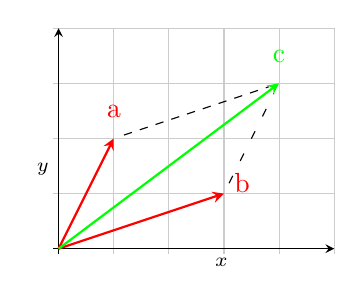
\begin{tikzpicture}%
\begin{scope}[scale=.7, rotate=0]
  \draw[thin,gray!40] (-0.1,-0.1) grid (5,4);
  \draw[-stealth] (-0.1,0)--(5,0) node[midway, below, xshift=10]{${\scriptstyle x}$};
  \draw[-stealth] (0,-0.1)-- (0,4) node[midway, left, yshift=-10]{${\scriptstyle y}$};
%  \draw[line width=.1pt ,black] ([shift=(0:5)]0,0) arc (0:90:5);
%  \draw[thick, blue, -stealth](0,0)--($cos(\ojobangle-\ojfrangle)*(5,0)$) node(x){};
%  \draw[thick, blue, -stealth](0,0)--($sin(\ojobangle-\ojfrangle)*(0,5)$) node(y){};
  \draw[thick, red, -stealth](0,0)--(1,2) node[label={[above]\vect{a}}] (A){};
  \draw[thick, red, -stealth](0,0)--(3,1) node[label={[right]\vect{b}}] (B){};
  \draw[thick, green, -stealth](0,0)--(4,3) node[label={[above]\vect{c}}] (C){};
  \draw[ dashed] (A)--(C);
  \draw[loosely dashed] (B)--(C);
\end{scope}
\end{tikzpicture}
\captionof{figure}{Optellen van vectoren. \label {fig:vectorsom}}}
\iffalse%_+
\marginnote{\vspace{5cm}\includegraphics[width=0.95\marginparwidth]{./img/vectorsom.png}
 \captionof{figure}{Optellen van vectoren.
Parallellogram-methode of kop aan staart methode. Maar ook is mogelijk: x-componenten optellen en y-componenten optellen.
 \label {fig:vectorsom}}}
\fi%_+
Door van een vector de co\"ordinaten te geven ligt die vector vast. 
Op grond van de overwegingen bij figuur~\ref{fig:vectorsom} gaan we een vector weergeven m.b.v. zijn componenten. Dus $A$ door bijvoorbeeld
$\mqty(a\\b)$en $B$ door bijvoorbeeld
$\mqty(c\\d)$.

Voor de som van de twee vectoren $A$ en $B$ nemen we dan als definitie:
$$C =  A +  B  = 
\mqty(a\\b)+\mqty(c\\d)=\mqty(a+c\\b+d)$$  

\subsection*{Co\"ordinatentransformaties}
Voor de definitie van de vectorsom hebben we gebruik gemaakt van co\"ordinaten. Een co\"ordinatensysteem is altijd nodig om kwantitatieve uitspraken te doen over fysische grootheden die zich gedragen als vectoren. Voor zo'n systeem van co\"ordinaten is een basis nodig. Die basis wordt gevormd door twee vectoren met lengte \'e\'en die loodrecht op elkaar staan. 
De keuze van de basis is vrij. Bekijk figuur~\ref{fig:anderebasis}. De vectoren \vect{a} en \vect{b} zijn daar weergegeven in twee co\"ordinatensystemen elk met hun eigen basis.

\iffalse%-=
\begin{center}
\leavevmode
\includegraphics[width=0.95\textwidth]{./img/anderebasis.png}
 \captionof{figure}{Twee vectoren. De keuze van het co\"ordinatensysteem is vrij. 
Bij een transformatie van het ene co\"ordinaten-systeem naar het andere blijven lengte en richting van de vectoren behouden. \label {fig:anderebasis}}
\end{center}
\fi%-=
\begin{minipage}{\textwidth}% to keep image and caption on one page
\makebox[\textwidth]{%        to center the image
\def\ojfrangle{0}
\def\ojobangle{70}
\def\ojscale{.75}
\begin{tikzpicture}%
\begin{scope}[scale=\ojscale, rotate=\ojfrangle]
\node at (4,3) {E};
  \draw[thin,red!40] (-0.1,-0.1) grid (4,3);

  \draw[-stealth, red] (0,0)--(1,0) node[midway, below, xshift=0]{${\scriptstyle e_1}$};
  \draw[-stealth, red] (0,0)-- (0,1) node[midway, left, yshift=0]{${\scriptstyle e_2}$};
%  \draw[line width=.1pt ,black] ([shift=(0:5)]0,0) arc (0:90:5);
%  \draw[thick, blue, -stealth](0,0)--($cos(\ojobangle-\ojfrangle)*(5,0)$) node(x){};
%  \draw[thick, blue, -stealth](0,0)--($sin(\ojobangle-\ojfrangle)*(0,5)$) node(y){};
%  \draw[thick, red, -stealth](0,0)--(1,2) node[label={[above]a}] (A){};
  \draw[thick, blue, -stealth](0,0)--(1,2) node[label={[above]$\vec{a} \smqty(1\\2)$}] (p){};
  \draw[thick, blue, -stealth](0,0)--(3,1) node[label={[above]$\vec{b} \smqty(3\\1)$}] (q){};

  \filldraw[fill=blue!20!white, draw=blue!10!black] (0,0) -- (18.43:1cm)
    arc [start angle=18.43, end angle=63.43, radius=10mm] -- cycle;
\node at (1,1){$\phi$};
%  \draw[loosely dashed] (x)--(p);

%  \draw[loosely dashed] (y)--(p);
\end{scope}
%  \node [below] at (0,0) {$1$};
\end{tikzpicture}
\def\ojfrangle{63.43-90}
\begin{tikzpicture}
\begin{scope}[scale=\ojscale,  rotate=\ojfrangle]
\node at (4,3) {J};
  \draw[thin,green!40] (-0.1,-0.1) grid (4,3);
  \draw[-stealth, green] (0,0)--(1,0) node[midway, below, xshift=0]{${\scriptstyle j_1}$};
  \draw[-stealth, green] (0,0)-- (0,1) node[midway, left, yshift=5]{${\scriptstyle j_2}$};
%  \draw[line width=.1pt ,black] ([shift=(0:5)]0,0) arc (0:90:5);
%  \draw[thick, blue, -stealth](0,0)--($cos(\ojobangle-\ojfrangle)*(5,0)$) node(x){};
%  \draw[thick, blue, -stealth](0,0)--($sin(\ojobangle-\ojfrangle)*(0,5)$) node(y){};
  \draw[thick, blue, -stealth](0,0)--(0,2.236) node[label={[right]$\vec{a}\smqty(0\\\sqrt{5})$}] (p){};
  \draw[thick, blue, -stealth](0,0)--(2.236,2.236) node[label={[right]$\vec{b}\smqty(\sqrt{5}\\\sqrt{5})$}] (q){};

  \filldraw[fill=blue!20!white, draw=blue!50!black] (0,0) -- (45:1cm) 
    arc [start angle=45, end angle=90, radius=10mm] -- cycle;
\node at((0.5,1.4){$\phi$};
%  \draw[loosely dashed] (x)--(p);
%  \draw[loosely dashed] (y)--(p);
\end{scope}
%  \node [below] at (0,0) {$2$};
\end{tikzpicture}
}
\captionof{figure}{Twee vectoren. De keuze van het co\"ordinatensysteem is vrij. 
Bij een transformatie van het ene co\"ordinaten-systeem naar het andere blijven lengte en richting van de vectoren behouden. \label{fig:anderebasis}}
\end{minipage}

\bigskip
Intu\"itief lijkt bij de overgang van basis $E$ naar basis $J$ weinig te veranderen. Alleen het ruitjespatroon is gedraaid en er zijn twee nieuwe vectoren in beeld gekomen: de basisvectoren $\vect{j_1}$  en $\vect{j_2}$. Je bent vrij in je keuze. Vaak is de  combinatie van 
een horizontale en een verticale as  handig maar niet altijd.  De keuze van een co\"ordinatensysteem vindt plaats door twee onderling loodrechte vectoren met lengte \'e\'en te kiezen. In de twee-dimensionele ruimte vormen die dan een  basis.
Noemen we de twee basisvectoren $\vect{e_1}$ en  $\vect{e_2}$, dan geldt voor een willekeurige vector $\vect{v}$.
$$\vect{v}  = \alpha\vect{e_1} + \beta\vect{e_2}$$
De weergave van de vector $\vect{v}$ in die basis is dan $\mqty(\alpha\\\beta)$.
Alle vectoren $\vect{v}$ vullen dan die tweedimensionale ruimte. In figuur~\ref{fig:anderebasis} is dat voor twee keuzes van een basis gedaan. Dat zijn de bases $E$ en $J$.%einde van dit wiskunde kader
\end{mdframed}%
\begin{antwoord}
\begin{enumerate}[left=-3pt]
\item $\vect{j_1}=\smqty(1\\0)$\\$j_2=\smqty(0\\1)$
\item $\frac{1}{5}\sqrt{5}\smqty(1\\2)$
\item $\vect{e_1}=\frac{1}{5}\sqrt{5}\smqty(2\\1)$\\$ e_2=\frac{1}{5}\sqrt{5}\smqty(-1\\2)$
\item $\norm{A}=\sqrt{5}$    $\norm{B}=\sqrt(10)$
\end{enumerate}
\end{antwoord}
\begin{opdracht}[red]%
Bekijk figuur~\ref{fig:anderebasis}.
\begin{enumerate}[noitemsep]
\item Wat zijn de componenten van de vectoren $\vect{j_1}$ en $\vect{j_2}$ in basis $J$?
\end{enumerate}
In basis $E$ geldt: $\vect{j_2} =\mqty(\alpha\\\beta)$. 
\begin{enumerate}[noitemsep,resume]
\item Bereken $\alpha$ en $\beta$ met behulp van vector $\vect{a}$ in figuur~\ref{fig:anderebasis}.
\item Geef de componenten van de vectoren $\vect{e_1}$ en $\vect{e_2}$ in basis $J$.
\item Bepaal de lengte van beide vectoren $\vect{a}$ en $\vect{b}$.
\item Vul tabel~\ref{table:tabelEJ} in.
\end{enumerate}
\end{opdracht}
In tabel~\ref{table:tabelEJ} zijn de resultaten nog eens weergegeven. 
%------------
%\leavevmode
{\renewcommand{\arraystretch}{2}%--__--__
\begin{tabular}{|l|l|l|}\hline
\multicolumn{3}{|c|}{%==-=-=-=--=-=-=-=-=-=-=-
\def\ojfrangle{0}
\def\ojobangle{70}
\def\ojscale{.75}
\begin{tikzpicture}%
\begin{scope}[scale=\ojscale, rotate=\ojfrangle]
\node at (4,3) {E};
  \draw[thin,red!20] (-0.1,-0.1) grid (4,3);

  \draw[-stealth, red] (0,0)--(1,0) node[midway, below]{${\scriptstyle e_1}$};
  \draw[-stealth, red] (0,0)-- (0,1) node[midway, left]{${\scriptstyle{e_2}}$};
%  \draw[line width=.1pt ,black] ([shift=(0:5)]0,0) arc (0:90:5);
%  \draw[thick, blue, -stealth](0,0)--($cos(\ojobangle-\ojfrangle)*(5,0)$) node(x){};
%  \draw[thick, blue, -stealth](0,0)--($sin(\ojobangle-\ojfrangle)*(0,5)$) node(y){};
%  \draw[thick, red, -stealth](0,0)--(1,2) node[label={[above]a}] (A){};
  \draw[thick, blue, -stealth](0,0)--(1,2) node[label={[red, above]$\smqty(1\\2)$}] (p){};
  \draw[thick, blue, -stealth](0,0)--(3,1) node[label={[red, above]$\smqty(3\\1)$}] (q){};
  \node[blue,left] at (1,2) {$\vect{a}$};
  \node[blue,below] at (3,1) {$\vect{b}$};
  \filldraw[fill=blue!20!white, draw=blue!10!black] (0,0) -- (18.43:1cm)
    arc [start angle=18.43, end angle=63.43, radius=10mm] -- cycle;
\node at((1,1){$\phi$};
%  \draw[loosely dashed] (x)--(p);
%  \draw[loosely dashed] (y)--(p);
\end{scope}
%  \node [below] at (0,0) {$1$};
%\end{tikzpicture}
%&
\def\ojfrangle{63.43-90}%cos(1/sqrt5)=63.34 deg
%\def\ojobangle{70}
%\def\ojscale{.75}
%\begin{tikzpicture}
\begin{scope}[scale=\ojscale,  rotate=\ojfrangle]
\node at (4,3) {J};
  \draw[thin,green!40] (-0.1,-0.1) grid (4,3);
  \draw[-stealth, red] (0,0)--(90-63.43:1) node[midway, below, xshift=0]{${\scriptstyle e_1}$};
  \draw[-stealth, red] (0,0)-- (180-63.43:1) node[midway, left, yshift=0]{${\scriptstyle e_2}$};
  \draw[-stealth, green] (0,0)--(1,0) node[midway, below, xshift=0]{${\scriptstyle j_1}$};
  \draw[-stealth, green] (0,0)-- (0,1) node[midway, left, yshift=5]{${\scriptstyle j_2}$};
%  \draw[line width=.1pt ,black] ([shift=(0:5)]0,0) arc (0:90:5);
%  \draw[thick, blue, -stealth](0,0)--($cos(\ojobangle-\ojfrangle)*(5,0)$) node(x){};
%  \draw[thick, blue, -stealth](0,0)--($sin(\ojobangle-\ojfrangle)*(0,5)$) node(y){};
  \draw[thick, blue, -stealth](0,0)--(0,2.236) node[label={[green, right]$\smqty(0\\\sqrt{5})$}] (p){};
  \draw[thick, blue, -stealth](0,0)--(2.236,2.236) node[label={[green, right]${\smqty(\sqrt{5}\\\sqrt{5})}$}] (q){};
%  \filldraw[fill=green!20!white, draw=green!50!black] (0,0) -- (45:1cm) 
%    arc [start angle=45, end angle=90, radius=10mm] -- cycle;
%\node at((0.5,1.4){$\phi$};
%  \draw[loosely dashed] (x)--(p);
%  \draw[loosely dashed] (y)--(p);
\end{scope}
%  \node [below] at (0,0) {$2$};
\end{tikzpicture}
}\\\hline%=-=-=-=-=-=-=-=-=-=-=-=-
& in $E$ & in $J$ \\ \hline
\cellcolor{red!40}$\vect{e_1}$ &\cellcolor{red!40}$\smqty(1\\0)$  &\cellcolor{red!40}$\tfrac{1}{\sqrt{5}}\smqty(2\\1)$\\ \hline
\cellcolor{red!40}$\vect{e_2}$ &\cellcolor{red!40}$\smqty(0\\1)$        &\cellcolor{red!40}
%%%%$\tfrac{1}{\sqrt{5}}\smqty(-1\\2)$
\\ \hline
\cellcolor{green!40}$\vect{j_1}$ &\cellcolor{green!40}
%%%%$\tfrac{1}{\sqrt{5}}\smqty(2\\-1)$
&\cellcolor{green!40}$\smqty(1\\0)$        \\ \hline
\cellcolor{green!40}$\vect{j_2}$ &\cellcolor{green!40}
%%%%$\tfrac{1}{\sqrt{5}}\smqty(1\\2)$
&\cellcolor{green!40}$\smqty(0\\1)$\\ \hline
\cellcolor{gray!10}$A$&\cellcolor{gray!10}$\smqty(1\\2)=1\smqty(1\\0)+2\smqty(0\\1)$&\cellcolor{gray!10}
%%%%$\tfrac{1}{\sqrt{5}}\smqty(0\\5)$
%$\mqty(0\\\sqrt{5})$%=0\mqty(1\\0)+\sqrt{5}\mqty(0\\1)$
\\ \hline
\cellcolor{gray!10}$B$&\cellcolor{gray!10}$\smqty(3\\1)=3\smqty(1\\0) +1\smqty(0\\1)$
&\cellcolor{gray!10}
\hspace{3cm}
%%%%$\tfrac{1}{\sqrt{5}}\smqty(5\\5)$
\\ \hline
%%%%\cellcolor{gray!40}$C$&\cellcolor{gray!40}$\smqty(1\\2)+\smqty(3\\1) = \smqty(4\\3)$&\cellcolor{gray!40}$\smqty(0\\\sqrt{5})+0\smqty(\sqrt{5}\\\sqrt{5}) \equiv \smqty(\sqrt{5}\\2\sqrt{5})$\\ \hline
\end{tabular}
}%--__--__
 \captionof{table}{Twee bases
 \label{table:tabelEJ}}
\begin{antwoord}[-9cm]
\begin{enumerate}[left=-3pt]
\setcounter{enumi}{4}\item $e_{2_J}=\tfrac{1}{5}\sqrt{5}\smqty(-1\\2)$\\
$j_{1_E}=\tfrac{1}{5}\sqrt{5}\smqty(2\\-1)$\\
$j_{2_E}=\tfrac{1}{5}\sqrt{5}\smqty(1\\2)$\\
$e_{1_J}=\tfrac{1}{2}\sqrt{5}\smqty(2\\1)$\\
$e_{2_J}=\tfrac{1}{2}\sqrt{5}\smqty(-1\\2)$\\
$\smqty(1\\1)=1\smqty(1\\0)+2\smqty(0\\1)$=\\
$\smqty(0\\\sqrt{5})$\\
$\smqty(3\\1)=3\smqty(1\\0)+1\smqty(0\\1)$=\\
$\smqty(\sqrt{5}\\\sqrt{5})$
\end{enumerate}
\end{antwoord}
\end{document}